\subsection{Centro}

  \paragraph{}Se procede a crear el centro al que pertenecen tanto el alumno
  como el asesor, en este caso \textit{Facultad de Ciencias}. Para ello, se
  realizará la creación de un nuevo centro, tal y como se describió en el
  capítulo \ref{addCentro}, \textit{Añadir centro}.

  \paragraph{}Una vez que aparezca el formulario de creación, se debe introducir
  el nombre del centro, con lo que la pantalla quedaría tal y como refleja la
  figura \ref{ejemploAddCentro}.

  \begin{figure}[!ht]
    \begin{center}
      \fbox{
      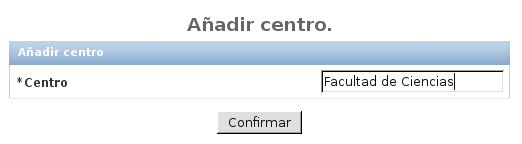
\includegraphics[scale=0.55]{5.Ejemplos_Practicos/5.3.IntroduccionDatos/5.3.1.Centro/add_centro.png}
      }
      \caption{Creación de \textit{Centro} de ejemplo.}
      \label{ejemploAddCentro}
    \end{center}
  \end{figure}
